\documentclass[border=2mm]{standalone}
\usepackage{pgfplots}
\usepgfplotslibrary{groupplots}
\pgfplotsset{compat=1.18}
\definecolor{BCred}{rgb}{0.7, 0.11, 0.11}
\definecolor{BCblue}{rgb}{0.0, 0.20, 0.42}
\definecolor{BCgreen}{rgb}{0.11, 0.35, 0.02}
\pgfplotsset{every axis/.append style={width=7.5cm, height=7.5cm, scale only axis,
  ticklabel style={font=\small, /pgf/number format/fixed},
  yticklabel style={text width=10mm, align=right},
  label style={font=\normalsize}, title style={font=\normalsize},
  legend style={draw=none, font=\small}}}
\begin{document}
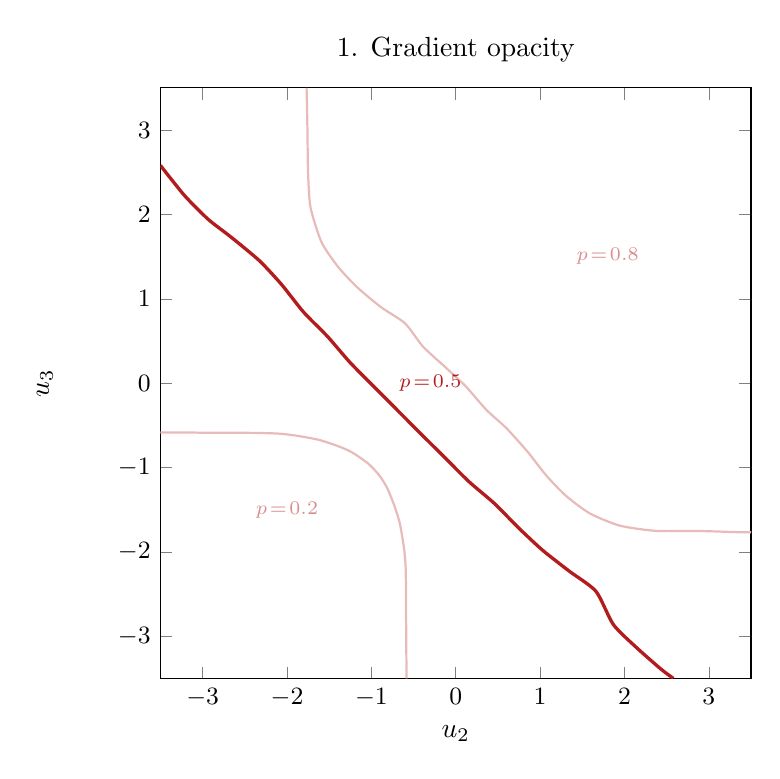
\begin{tikzpicture}
\begin{groupplot}[group style={group size=1 by 1}]
\nextgroupplot[xmin=-3.5, xmax=3.5, ymin=-3.5, ymax=3.5, xlabel={$u_2$}, ylabel={$u_3$}, axis equal image, title={1. Gradient opacity}]
\addplot[thick,color=BCred!30,smooth,tension=0.4] coordinates {(-3.500,-0.584)(-3.217,-0.585)(-2.934,-0.588)(-2.652,-0.589)(-2.369,-0.590)(-2.086,-0.599)(-1.874,-0.625)(-1.623,-0.672)(-1.408,-0.742)(-1.237,-0.816)(-1.036,-0.955)(-0.904,-1.096)(-0.813,-1.243)(-0.729,-1.449)(-0.663,-1.662)(-0.615,-1.944)(-0.595,-2.157)(-0.590,-2.439)(-0.589,-2.722)(-0.587,-3.005)(-0.585,-3.288)(-0.584,-3.500)};
\addplot[very thick,color=BCred,smooth,tension=0.4] coordinates {(-3.500,2.580)(-3.218,2.227)(-2.937,1.944)(-2.652,1.722)(-2.325,1.449)(-2.063,1.167)(-1.803,0.841)(-1.520,0.553)(-1.255,0.247)(-0.976,-0.035)(-0.695,-0.318)(-0.413,-0.601)(-0.128,-0.884)(0.156,-1.167)(0.460,-1.428)(0.742,-1.713)(1.025,-1.977)(1.343,-2.227)(1.662,-2.468)(1.870,-2.864)(2.155,-3.146)(2.439,-3.395)(2.580,-3.500)};
\addplot[thick,color=BCred!30,smooth,tension=0.4] coordinates {(-1.768,3.500)(-1.758,3.005)(-1.751,2.510)(-1.722,2.086)(-1.591,1.670)(-1.395,1.379)(-1.167,1.135)(-0.884,0.899)(-0.601,0.709)(-0.389,0.434)(-0.110,0.177)(0.116,-0.035)(0.364,-0.318)(0.601,-0.534)(0.851,-0.813)(1.074,-1.096)(1.308,-1.337)(1.591,-1.545)(1.944,-1.689)(2.369,-1.751)(2.864,-1.752)(3.359,-1.767)(3.500,-1.768)};
\node[font=\scriptsize,color=BCred!50] at (axis cs:-2.0,-1.5) {$p\!=\!0.2$};
\node[font=\scriptsize,color=BCred] at (axis cs:-0.3,0.0) {$p\!=\!0.5$};
\node[font=\scriptsize,color=BCred!50] at (axis cs:1.8,1.5) {$p\!=\!0.8$};
\end{groupplot}
\end{tikzpicture}
\end{document}
